%==============================================================================
%  Building GPT-2 from Scratch — Interpretive Summary (max 3 pages)
%  CENG-534, Izmir Institute of Technology (IZTECH)
%  Build:  tectonic summary.tex   (or: pdflatex summary)
%  Self-contained: no external .sty / .bib needed.
%==============================================================================
\documentclass[11pt]{article}

\usepackage[T1]{fontenc}
\usepackage[utf8]{inputenc}
\usepackage[margin=1in]{geometry}
\usepackage{times}
\usepackage{amsmath}
\usepackage{booktabs}
\usepackage{graphicx}
\usepackage{caption}
\usepackage[hidelinks]{hyperref}
\captionsetup{font=small}

\setlength{\parskip}{0.5em}
\setlength{\parindent}{0pt}

\title{\vspace{-3em}Building GPT-2 from Scratch: What We Learned}
\author{Hasan Semih Sel\c{c}uk \quad Matin Huseynzade \\
  \small Dept.\ of Computer Engineering, IZTECH. CENG-534 Default Final Project}
\date{}

\begin{document}
\maketitle
\vspace{-1.5em}

We set out to do two things: understand GPT-2 by rebuilding it from its
primitives, and then learn what it takes to bend a single pretrained model toward
tasks of increasing difficulty. In hindsight the project taught us less about any
one accuracy number and more about a recurring distinction between
\emph{recognizing} a property of text and \emph{producing} text that has it. It
also taught us how much of practical NLP lives in details that have nothing to do
with the model itself. This note records what we take away rather than a
slide-by-slide account; the full report carries every table and command.

\begin{table}[h]
\centering
\small
\begin{tabular}{@{}lll@{}}
\toprule
\textbf{Task} & \textbf{Setup} & \textbf{Result (dev / held-out)} \\
\midrule
Sentiment (CFIMDB) & full-model fine-tune & accuracy \textbf{0.967} (vs.\ 0.857 head-only) \\
Sentiment (SST-5)  & full-model fine-tune & accuracy 0.513 \\
Paraphrase (Quora) & cloze next-token, 3 epochs & accuracy \textbf{0.889} \\
Sonnet generation  & temperature sweep, top-$p$ 0.9 & chrF \textbf{41.49} at $\tau=1.0$ \\
Extension (mod.\,$\rightarrow$\,Shak.) & fine-tune + source-side masking & chrF \textbf{35.83} (13.85 zero-shot, $+21.97$) \\
\bottomrule
\end{tabular}
\caption{Our results on the course dev / held-out splits. Every number is our own
measurement and reproduces from committed artifacts (see end).}
\end{table}

\paragraph{Building the model was the cheap part; adapting it was the lesson.}
Writing masked attention, the pre-LayerNorm block, and a decoupled-weight-decay
AdamW by hand, and then watching the course tests pass, was satisfying but
mechanical. The interesting work began at fine-tuning. Our four tasks form a
deliberate progression (sentiment classification, paraphrase detection, sonnet
generation, and our extension), and each step up that ladder forced a new kind of
decision. Classification only asks the model to read. Generation asks it to commit
to an output distribution token by token, where small choices compound. The same
backbone served all four, which we read as evidence that the value of a pretrained
model is less in any task head and more in what transfers underneath.

\paragraph{Paraphrase: the framing mattered more than the tuning.} We treated the
binary Quora task not as a classifier with a new head but as a fill-in-the-blank
question, where the model simply prefers \texttt{yes} or \texttt{no} as the next
token, and reached $0.889$ dev accuracy. What stayed with us was not the number
but two quiet failure modes. Using even a slightly different prompt at test time
than at training time made dev look healthy while the held-out score quietly
collapsed. And na\"ively truncating long inputs from the right threw away the very
end of the prompt, where the answer is decided. Both bugs are invisible in the
loss curve. The lesson we drew is that when a task is posed as language modeling,
the prompt \emph{is} part of the model, and inconsistencies in it are as damaging
as a wrong hyperparameter.

\paragraph{Generation taught us to read a metric skeptically.} For sonnets we
condition on three lines and sample the rest, and a temperature sweep reproduced,
on our own model, the textbook degeneration/divergence trade-off: too cold and the
model loops, too hot and it wanders, with $\tau{=}1.0$ best at chrF $41.49$. But
the gaps between settings were small enough that we stopped treating chrF as
ground truth. chrF rewards $n$-gram overlap, exactly the signal that
over-confident, repetitive text can inflate, so we cross-checked with held-out
perplexity, which fine-tuning roughly halved ($99.1\rightarrow59.0$), and with
corpus-level diversity, which moved in the direction the chrF trend implied. The
habit we are taking forward is to never let a single generation metric stand
alone.

\begin{figure}[h]
\centering
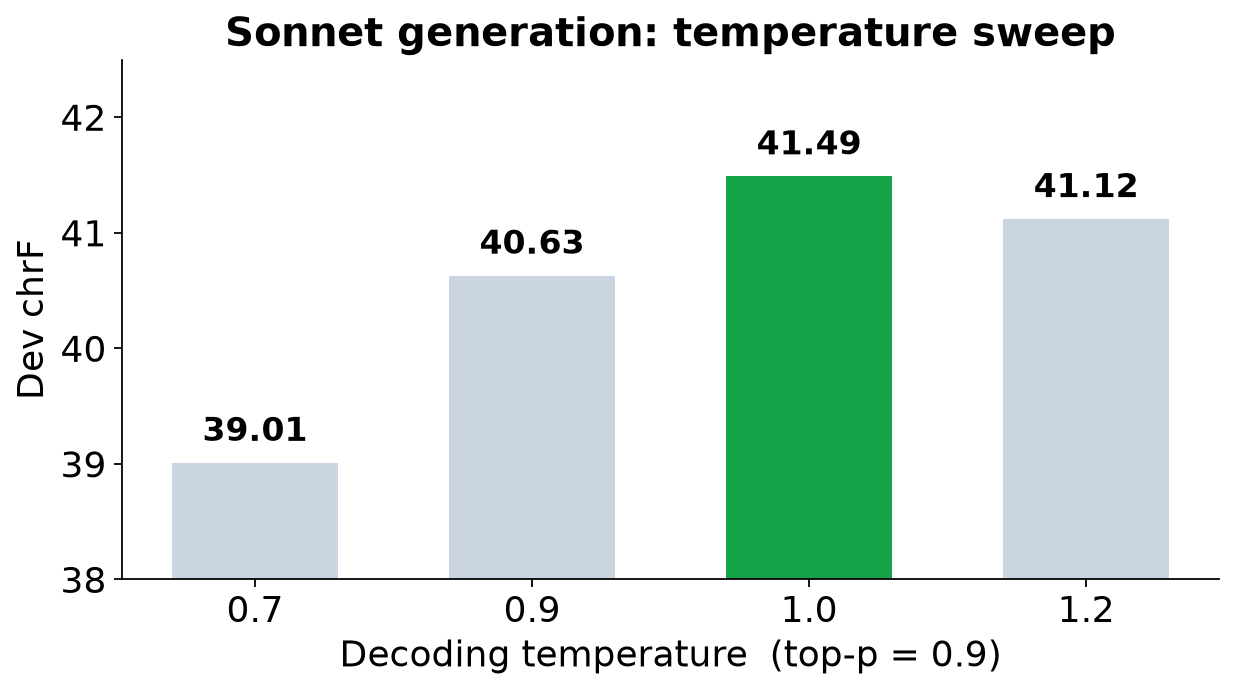
\includegraphics[width=0.62\linewidth]{figs/sonnet_temp.png}
\caption{Sonnet decoding-temperature sweep (dev chrF, top-$p$ fixed at $0.9$). The
ordering is clear but the spread is narrow, which is why we did not over-read it.}
\end{figure}

\paragraph{The extension: a small idea, isolated cleanly.} Our original
contribution rewrites modern English into Shakespearean style. We deliberately
introduced \emph{no new model class}: we reused the sonnet generator and changed
only the data and the loss, masking the source so the gradient comes from the
target tokens alone. This was a methodological choice as much as an engineering
one. By holding the architecture fixed, any improvement is attributable to data
and objective, not to a lucky new module. It worked: chrF more than doubled over
the zero-shot baseline ($13.85\rightarrow35.83$), and the outputs adopt archaic
morphology while preserving meaning, with failures dominated by harmless sampling
repetition rather than semantic drift.

\paragraph{The most useful finding came from the tokenizer, not the network.}
The single change with the highest return per character was deleting one space.
GPT-2's byte-pair encoding binds a leading space to the following token, so a
prompt ending in a space pushes the very first generation step
out-of-distribution; our model responded with strings of junk before recovering.
Moving that space from the prompt onto the target was worth $+6.3$ chrF. We
highlight this because it reframes where effort pays off. Understanding the
tokenizer's conventions returned more than any tuning we did to the model itself,
and it is the kind of bug that no validation accuracy would have flagged.

\begin{figure}[h]
\centering
\begin{minipage}{0.49\linewidth}\centering
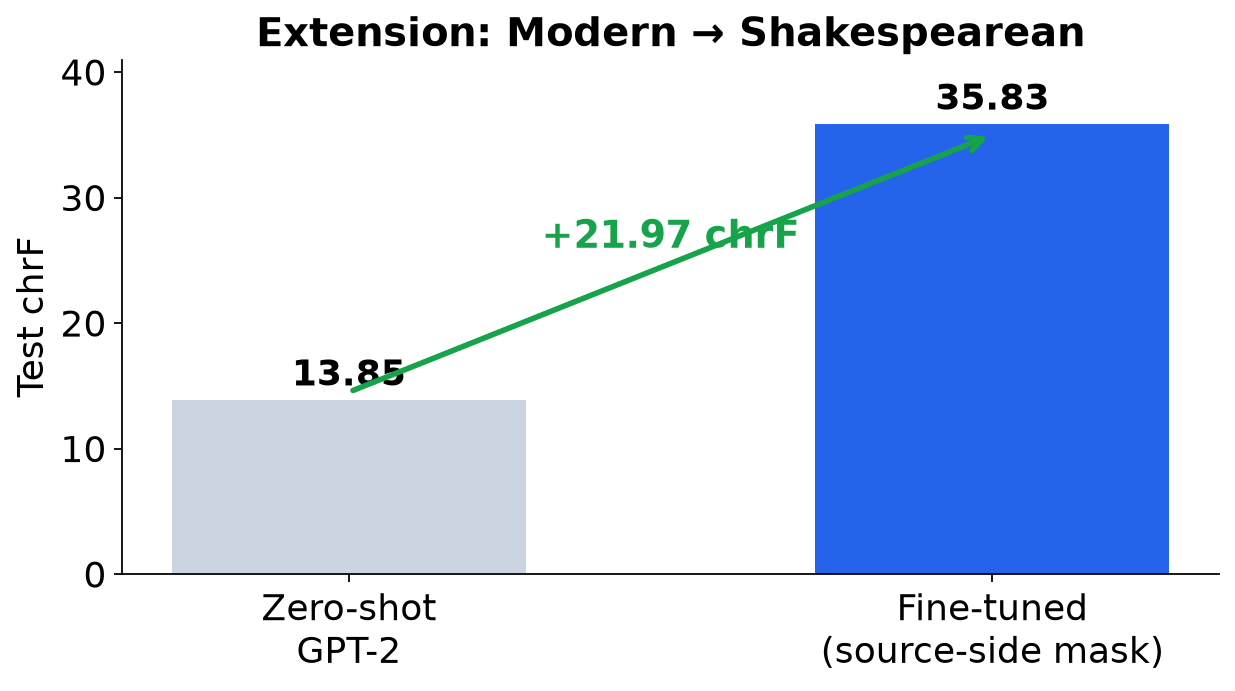
\includegraphics[width=\linewidth]{figs/extension.png}
\end{minipage}\hfill
\begin{minipage}{0.49\linewidth}\centering
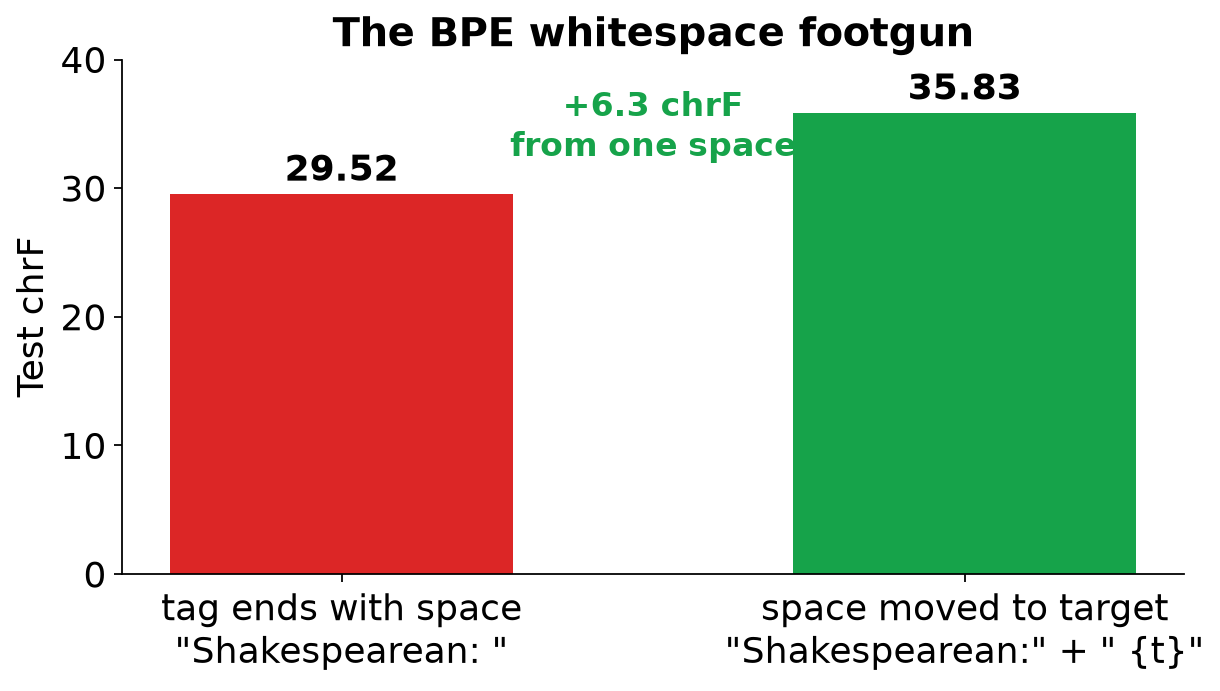
\includegraphics[width=\linewidth]{figs/prompt_ablation.png}
\end{minipage}
\caption{Left: the extension more than doubles chrF over zero-shot GPT-2. Right:
of the fine-tuned gain, $6.3$ chrF came from a single space moved off the prompt
tag, the tokenizer finding above.}
\end{figure}

\paragraph{Hardware was a real constraint, and it disciplined our claims.}
Everything was trained on an Apple M4 Pro with no CUDA GPU, on the MPS backend,
where variable-length batches fragment the allocator and eventually crash. The
recipe that made full fine-tuning stable (bounding sequence length, small batches,
periodic cache clearing, evaluation under \texttt{no\_grad}) is not novel, but
living under that ceiling changed how we reported results. The clearest example is
the one place we trail the handout (CFIMDB full, $0.967$ vs.\ $0.976$). The
tempting story is that our memory-forced small batch caused it. We tested that
story with a controlled gradient-accumulation experiment and it did not hold: a
larger effective batch did not close the gap within the same budget. So we report
the gap as unexplained rather than blame a convenient culprit. Testing a
hypothesis and finding it false felt like the most honest paragraph in the work.

\paragraph{What we would not claim, and what we would do next.} All our numbers
come from single runs, so we treat small differences as noise and would re-run
with multiple seeds and report variance before asserting any fine ranking. The
sonnet corpus is tiny and overfits within a couple of epochs. The natural next
step, and the one our hardware kept pointing at, is parameter-efficient
fine-tuning such as LoRA, which would relieve both the memory pressure and the
overfitting and let us move to a larger backbone. Beyond that, preference-based
tuning for sonnet quality and a richer generation metric such as MAUVE would
sharpen the evaluation. If the project has a single takeaway, it is that the
distance between a model that works and one that works \emph{well} was paved, for
us, with prompts, tokenizers, and memory, not with the architecture we started by
building.

\paragraph{Reproducibility.} Every number is regenerable in seconds from
committed artifacts, with no retraining, via \texttt{reproduce\_metrics.py}, which
re-scores the saved predictions against the gold labels.

\vspace{0.8em}
\hrule
\vspace{0.6em}
{\small Code, full report, and reproduction scripts:
\url{https://github.com/chillmatin/cs224n_gpt}}

\end{document}
